\definecolor{c82b366}{RGB}{130,179,102}
\definecolor{cd5e8d4}{RGB}{213,232,212}
\definecolor{c9673a6}{RGB}{150,115,166}
\definecolor{ce1d5e7}{RGB}{225,213,231}
\definecolor{c6c8ebf}{RGB}{108,142,191}
\definecolor{cdae8fc}{RGB}{218,232,252}
\definecolor{c666666}{RGB}{102,102,102}
\definecolor{whitesmoke}{RGB}{245,245,245}
\definecolor{c333333}{RGB}{51,51,51}


\def \globalscale {0.900000}
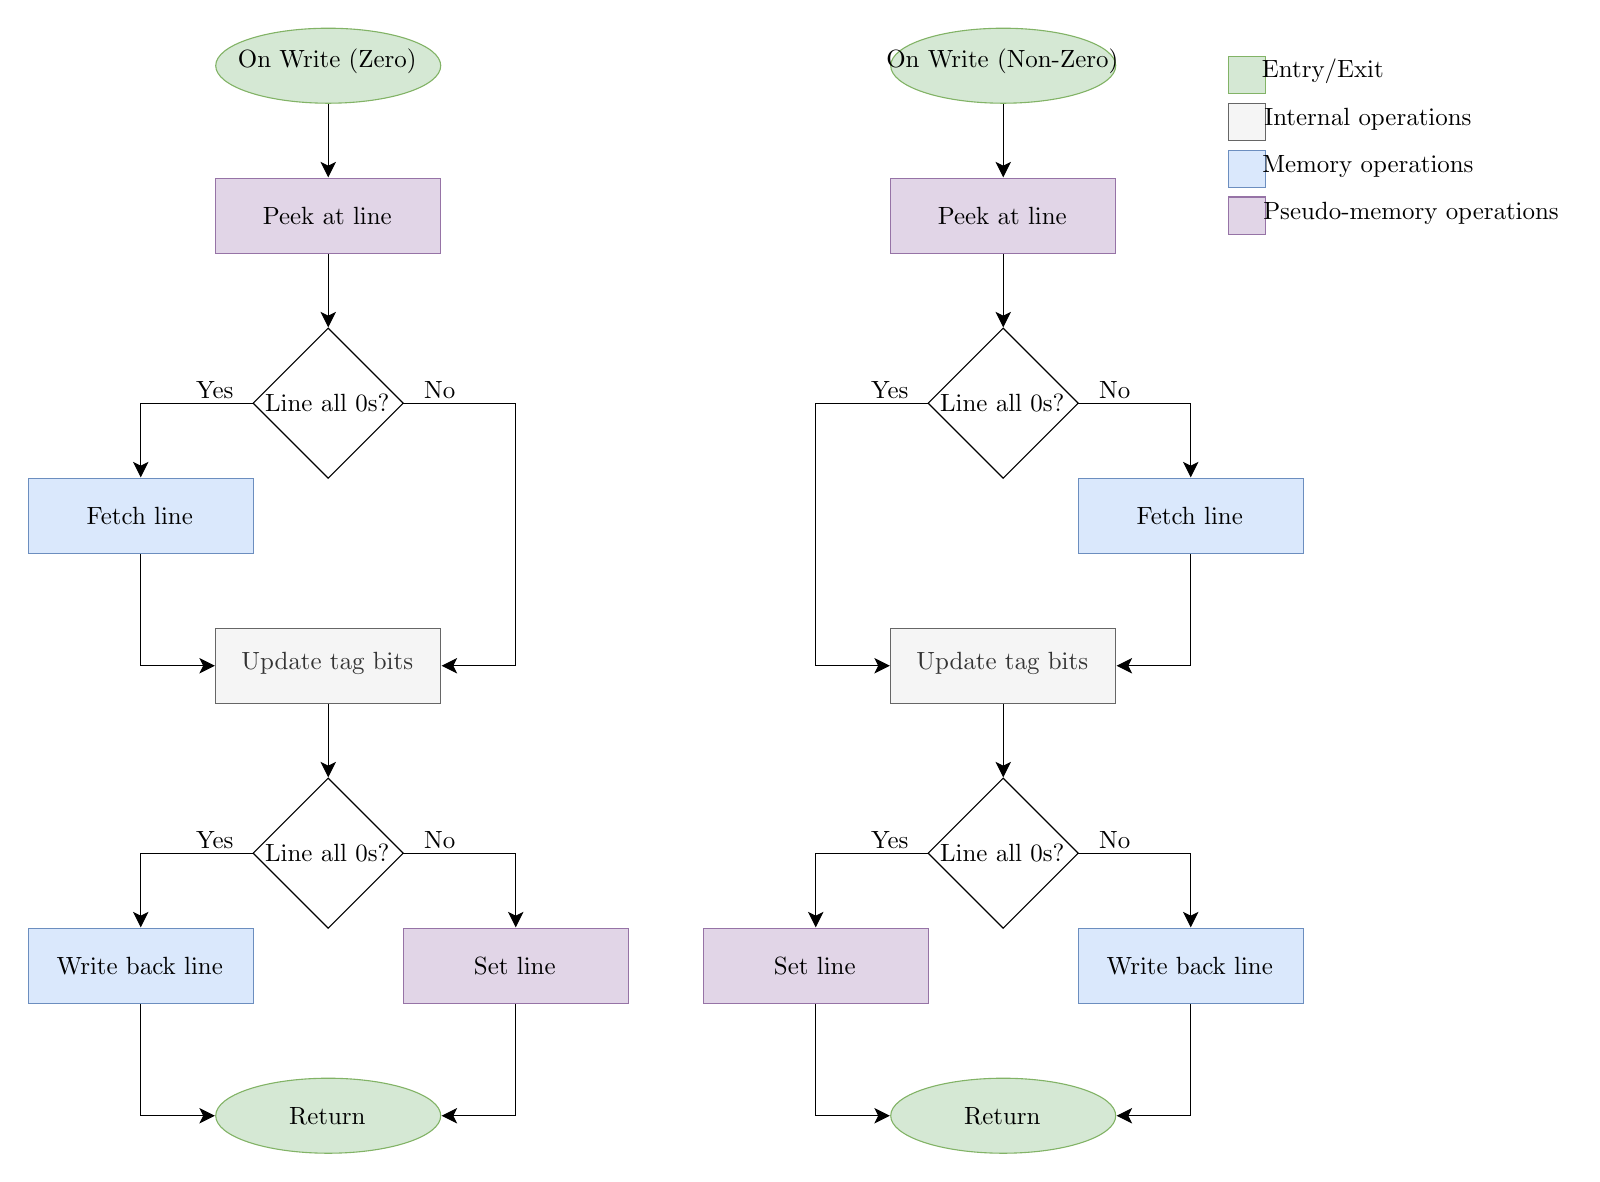
\begin{tikzpicture}[y=1cm, x=1cm, yscale=\globalscale,xscale=\globalscale, every node/.append style={scale=\globalscale}, inner sep=0pt, outer sep=0pt]
  \path[draw=black,miter limit=10.0] (4.2333, 14.8431) -- (4.2333, 14.314) -- (4.2333, 13.9533);



  \path[draw=black,fill=black,miter limit=10.0] (4.2333, 13.8144) -- (4.1407, 13.9996) -- (4.2333, 13.9533) -- (4.3259, 13.9996) -- cycle;



  \path[draw=c82b366,fill=cd5e8d4] (4.2333, 15.3723) ellipse (1.5875cm and 0.5292cm);



  \begin{scope}[fill=black,anchor=south]
    \node[text=black,anchor=south] (text7108) at (4.2201, 15.2532){On Write (Zero)};



  \end{scope}
  \path[draw=black,miter limit=10.0] (4.2333, 12.7265) -- (4.2333, 12.1973) -- (4.2333, 11.8367);



  \path[draw=black,fill=black,miter limit=10.0] (4.2333, 11.6978) -- (4.1407, 11.883) -- (4.2333, 11.8367) -- (4.3259, 11.883) -- cycle;



  \path[draw=c9673a6,fill=ce1d5e7] (2.6458, 13.7848) rectangle (5.8208, 12.7265);



  \begin{scope}[fill=black,anchor=south]
    \node[text=black,anchor=south] (text76) at (4.2201, 13.1366){Peek at line};



  \end{scope}
  \path[draw=black,miter limit=10.0] (1.5875, 8.4931) -- (1.5875, 6.9056) -- (2.4773, 6.9056);



  \path[draw=black,fill=black,miter limit=10.0] (2.6162, 6.9056) -- (2.431, 6.813) -- (2.4773, 6.9056) -- (2.431, 6.9982) -- cycle;



  \path[draw=c6c8ebf,fill=cdae8fc] (0.0, 9.5515) rectangle (3.175, 8.4931);



  \begin{scope}[fill=black,anchor=south]
    \node[text=black,anchor=south] (text5515) at (1.5743, 8.9032){Fetch line};



  \end{scope}
  \path[draw=black,miter limit=10.0] (3.175, 10.6098) -- (1.5875, 10.6098) -- (1.5875, 9.72);



  \path[draw=black,fill=black,miter limit=10.0] (1.5875, 9.5811) -- (1.4949, 9.7663) -- (1.5875, 9.72) -- (1.6801, 9.7663) -- cycle;



  \path[draw=black,miter limit=10.0] (5.2917, 10.6098) -- (6.8792, 10.6098) -- (6.8792, 6.9056) -- (5.9894, 6.9056);



  \path[draw=black,fill=black,miter limit=10.0] (5.8505, 6.9056) -- (6.0357, 6.9982) -- (5.9894, 6.9056) -- (6.0357, 6.813) -- cycle;



  \path[draw=black,fill=white,miter limit=10.0] (4.2333, 11.6681) -- (5.2917, 10.6098) -- (4.2333, 9.5515) -- (3.175, 10.6098) -- cycle;



  \begin{scope}[fill=black,anchor=south]
    \node[text=black,anchor=south] (text1946) at (4.2201, 10.4907){Line all 0s?};



  \end{scope}
  \path (2.1167, 11.1919) rectangle (3.175, 10.3981);



  \begin{scope}[fill=black,anchor=south]
    \node[text=black,anchor=south] (text3562) at (2.6326, 10.6759){Yes};



  \end{scope}
  \path (5.2917, 11.1919) rectangle (6.35, 10.3981);



  \begin{scope}[fill=black,anchor=south]
    \node[text=black,anchor=south] (text4963) at (5.8076, 10.6759){No};



  \end{scope}
  \path[draw=black,miter limit=10.0] (4.2333, 6.3765) -- (4.2333, 5.4867);



  \path[draw=black,fill=black,miter limit=10.0] (4.2333, 5.3478) -- (4.1407, 5.533) -- (4.2333, 5.4867) -- (4.3259, 5.533) -- cycle;



  \path[draw=c666666,fill=whitesmoke] (2.6458, 7.4348) rectangle (5.8208, 6.3765);



  \begin{scope}[fill=c333333,anchor=south]
    \node[text=c333333,anchor=south] (text4738) at (4.2201, 6.7866){Update tag bits};



  \end{scope}
  \path[draw=black,miter limit=10.0] (1.5875, 2.1431) -- (1.5875, 0.5556) -- (2.4773, 0.5556);



  \path[draw=black,fill=black,miter limit=10.0] (2.6162, 0.5556) -- (2.431, 0.463) -- (2.4773, 0.5556) -- (2.431, 0.6482) -- cycle;



  \path[draw=c6c8ebf,fill=cdae8fc] (0.0, 3.2015) rectangle (3.175, 2.1431);



  \begin{scope}[fill=black,anchor=south]
    \node[text=black,anchor=south] (text3656) at (1.5743, 2.5532){Write back line};



  \end{scope}
  \path[draw=black,miter limit=10.0] (3.175, 4.2598) -- (1.5875, 4.2598) -- (1.5875, 3.37);



  \path[draw=black,fill=black,miter limit=10.0] (1.5875, 3.2311) -- (1.4949, 3.4163) -- (1.5875, 3.37) -- (1.6801, 3.4163) -- cycle;



  \path[draw=black,miter limit=10.0] (5.2917, 4.2598) -- (6.8792, 4.2598) -- (6.8792, 3.37);



  \path[draw=black,fill=black,miter limit=10.0] (6.8792, 3.2311) -- (6.7866, 3.4163) -- (6.8792, 3.37) -- (6.9718, 3.4163) -- cycle;



  \path[draw=black,fill=white,miter limit=10.0] (4.2333, 5.3181) -- (5.2917, 4.2598) -- (4.2333, 3.2015) -- (3.175, 4.2598) -- cycle;



  \begin{scope}[fill=black,anchor=south]
    \node[text=black,anchor=south] (text9117) at (4.2201, 4.1407){Line all 0s?};



  \end{scope}
  \path (2.1167, 4.8419) rectangle (3.175, 4.0481);



  \begin{scope}[fill=black,anchor=south]
    \node[text=black,anchor=south] (text5729) at (2.6326, 4.3259){Yes};



  \end{scope}
  \path (5.2917, 4.8419) rectangle (6.35, 4.0481);



  \begin{scope}[fill=black,anchor=south]
    \node[text=black,anchor=south] (text8202) at (5.8076, 4.3259){No};



  \end{scope}
  \path[draw=c82b366,fill=cd5e8d4] (4.2333, 0.5556) ellipse (1.5875cm and 0.5292cm);



  \begin{scope}[fill=black,anchor=south]
    \node[text=black,anchor=south] (text6584) at (4.2201, 0.4366){Return};



  \end{scope}
  \path[draw=black,miter limit=10.0] (6.8792, 2.1431) -- (6.8792, 0.5556) -- (5.9894, 0.5556);



  \path[draw=black,fill=black,miter limit=10.0] (5.8505, 0.5556) -- (6.0357, 0.6482) -- (5.9894, 0.5556) -- (6.0357, 0.463) -- cycle;



  \path[draw=c9673a6,fill=ce1d5e7] (5.2917, 3.2015) rectangle (8.4667, 2.1431);



  \begin{scope}[fill=black,anchor=south]
    \node[text=black,anchor=south] (text2235) at (6.8659, 2.5532){Set line};



  \end{scope}
  \path[draw=black,miter limit=10.0] (13.7583, 14.8431) -- (13.7583, 14.314) -- (13.7583, 13.9533);



  \path[draw=black,fill=black,miter limit=10.0] (13.7583, 13.8144) -- (13.6657, 13.9996) -- (13.7583, 13.9533) -- (13.8509, 13.9996) -- cycle;



  \path[draw=c82b366,fill=cd5e8d4] (13.7583, 15.3723) ellipse (1.5875cm and 0.5292cm);



  \begin{scope}[fill=black,anchor=south]
    \node[text=black,anchor=south] (text847) at (13.7451, 15.2532){On Write (Non-Zero)};



  \end{scope}
  \path[draw=black,miter limit=10.0] (13.7583, 12.7265) -- (13.7583, 12.1973) -- (13.7583, 11.8367);



  \path[draw=black,fill=black,miter limit=10.0] (13.7583, 11.6978) -- (13.6657, 11.883) -- (13.7583, 11.8367) -- (13.8509, 11.883) -- cycle;



  \path[draw=c9673a6,fill=ce1d5e7] (12.1708, 13.7848) rectangle (15.3458, 12.7265);



  \begin{scope}[fill=black,anchor=south]
    \node[text=black,anchor=south] (text8339) at (13.7451, 13.1366){Peek at line};



  \end{scope}
  \path[draw=black,miter limit=10.0] (16.4042, 8.4931) -- (16.4042, 6.9056) -- (15.5144, 6.9056);



  \path[draw=black,fill=black,miter limit=10.0] (15.3755, 6.9056) -- (15.5607, 6.9982) -- (15.5144, 6.9056) -- (15.5607, 6.813) -- cycle;



  \path[draw=c6c8ebf,fill=cdae8fc] (14.8167, 9.5515) rectangle (17.9917, 8.4931);



  \begin{scope}[fill=black,anchor=south]
    \node[text=black,anchor=south] (text7416) at (16.3909, 8.9032){Fetch line};



  \end{scope}
  \path[draw=black,miter limit=10.0] (14.8167, 10.6098) -- (16.4042, 10.6098) -- (16.4042, 9.72);



  \path[draw=black,fill=black,miter limit=10.0] (16.4042, 9.5811) -- (16.3116, 9.7663) -- (16.4042, 9.72) -- (16.4968, 9.7663) -- cycle;



  \path[draw=black,miter limit=10.0] (12.7, 10.6098) -- (11.1125, 10.6098) -- (11.1125, 6.9056) -- (12.0023, 6.9056);



  \path[draw=black,fill=black,miter limit=10.0] (12.1412, 6.9056) -- (11.956, 6.813) -- (12.0023, 6.9056) -- (11.956, 6.9982) -- cycle;



  \path[draw=black,fill=white,miter limit=10.0] (13.7583, 11.6681) -- (14.8167, 10.6098) -- (13.7583, 9.5515) -- (12.7, 10.6098) -- cycle;



  \begin{scope}[fill=black,anchor=south]
    \node[text=black,anchor=south] (text5107) at (13.7451, 10.4907){Line all 0s?};



  \end{scope}
  \path (11.6417, 11.1919) rectangle (12.7, 10.3981);



  \begin{scope}[fill=black,anchor=south]
    \node[text=black,anchor=south] (text1447) at (12.1576, 10.6759){Yes};



  \end{scope}
  \path (14.8167, 11.1919) rectangle (15.875, 10.3981);



  \begin{scope}[fill=black,anchor=south]
    \node[text=black,anchor=south] (text1075) at (15.3326, 10.6759){No};



  \end{scope}
  \path[draw=black,miter limit=10.0] (13.7583, 6.3765) -- (13.7583, 5.4867);



  \path[draw=black,fill=black,miter limit=10.0] (13.7583, 5.3478) -- (13.6657, 5.533) -- (13.7583, 5.4867) -- (13.8509, 5.533) -- cycle;



  \path[draw=c666666,fill=whitesmoke] (12.1708, 7.4348) rectangle (15.3458, 6.3765);



  \begin{scope}[fill=c333333,anchor=south]
    \node[text=c333333,anchor=south] (text4668) at (13.7451, 6.7866){Update tag bits};



  \end{scope}
  \path[draw=black,miter limit=10.0] (11.1125, 2.1431) -- (11.1125, 0.5556) -- (12.0023, 0.5556);



  \path[draw=black,fill=black,miter limit=10.0] (12.1412, 0.5556) -- (11.956, 0.463) -- (12.0023, 0.5556) -- (11.956, 0.6482) -- cycle;



  \path[draw=c9673a6,fill=ce1d5e7] (9.525, 3.2015) rectangle (12.7, 2.1431);



  \begin{scope}[fill=black,anchor=south]
    \node[text=black,anchor=south] (text7616) at (11.0993, 2.5532){Set line};



  \end{scope}
  \path[draw=black,miter limit=10.0] (12.7, 4.2598) -- (11.1125, 4.2598) -- (11.1125, 3.37);



  \path[draw=black,fill=black,miter limit=10.0] (11.1125, 3.2311) -- (11.0199, 3.4163) -- (11.1125, 3.37) -- (11.2051, 3.4163) -- cycle;



  \path[draw=black,miter limit=10.0] (14.8167, 4.2598) -- (16.4042, 4.2598) -- (16.4042, 3.37);



  \path[draw=black,fill=black,miter limit=10.0] (16.4042, 3.2311) -- (16.3116, 3.4163) -- (16.4042, 3.37) -- (16.4968, 3.4163) -- cycle;



  \path[draw=black,fill=white,miter limit=10.0] (13.7583, 5.3181) -- (14.8167, 4.2598) -- (13.7583, 3.2015) -- (12.7, 4.2598) -- cycle;



  \begin{scope}[fill=black,anchor=south]
    \node[text=black,anchor=south] (text8833) at (13.7451, 4.1407){Line all 0s?};



  \end{scope}
  \path (11.6417, 4.8419) rectangle (12.7, 4.0481);



  \begin{scope}[fill=black,anchor=south]
    \node[text=black,anchor=south] (text8952) at (12.1576, 4.3259){Yes};



  \end{scope}
  \path (14.8167, 4.8419) rectangle (15.875, 4.0481);



  \begin{scope}[fill=black,anchor=south]
    \node[text=black,anchor=south] (text2228) at (15.3326, 4.3259){No};



  \end{scope}
  \path[draw=c82b366,fill=cd5e8d4] (13.7583, 0.5556) ellipse (1.5875cm and 0.5292cm);



  \begin{scope}[fill=black,anchor=south]
    \node[text=black,anchor=south] (text6707) at (13.7451, 0.4366){Return};



  \end{scope}
  \path[draw=black,miter limit=10.0] (16.4042, 2.1431) -- (16.4042, 0.5556) -- (15.5144, 0.5556);



  \path[draw=black,fill=black,miter limit=10.0] (15.3755, 0.5556) -- (15.5607, 0.6482) -- (15.5144, 0.5556) -- (15.5607, 0.463) -- cycle;



  \path[draw=c6c8ebf,fill=cdae8fc] (14.8167, 3.2015) rectangle (17.9917, 2.1431);



  \begin{scope}[fill=black,anchor=south]
    \node[text=black,anchor=south] (text5565) at (16.3909, 2.5532){Write back line};



  \end{scope}
  \path[draw=c82b366,fill=cd5e8d4] (16.9333, 15.5046) rectangle (17.4625, 14.9754);



  \path (17.3567, 15.6369) rectangle (19.2088, 14.8431);



  \begin{scope}[fill=black,anchor=south]
    \node[text=black,anchor=south] (text5102) at (18.2695, 15.1209){Entry/Exit};



  \end{scope}
  \path[draw=c666666,fill=whitesmoke] (16.9333, 14.8431) rectangle (17.4625, 14.314);



  \path (17.3302, 14.9754) rectangle (20.5052, 14.1817);



  \begin{scope}[fill=black,anchor=south]
    \node[text=black,anchor=south] (text884) at (18.9045, 14.4595){Internal operations};



  \end{scope}
  \path[draw=c6c8ebf,fill=cdae8fc] (16.9333, 14.1817) rectangle (17.4625, 13.6525);



  \path (17.1979, 14.314) rectangle (20.6375, 13.5202);



  \begin{scope}[fill=black,anchor=south]
    \node[text=black,anchor=south] (text1229) at (18.9045, 13.798){Memory operations};



  \end{scope}
  \path[draw=c9673a6,fill=ce1d5e7] (16.9333, 13.5202) rectangle (17.4625, 12.991);



  \path (17.2773, 13.6525) rectangle (21.7752, 12.8588);



  \begin{scope}[fill=black,anchor=south]
    \node[text=black,anchor=south] (text7633) at (19.513, 13.1366){Pseudo-memory operations};



  \end{scope}

\end{tikzpicture}
